% 建议使用 XeLaTeX 或 LuaLaTeX 编译(中文与公式支持更佳)
\documentclass[UTF8,zihao=-4]{ctexart}

\usepackage[a4paper,margin=2.5cm]{geometry}
\usepackage{amsmath, amssymb, amsthm}
\usepackage{bm}
\usepackage{hyperref}
\usepackage{graphicx}
\usepackage{caption}
\usepackage{listings}
\usepackage{xcolor}
\usepackage{float}
\usepackage{placeins}
\graphicspath{{figures/}}

\lstdefinestyle{code}{
  basicstyle=\ttfamily\small,
  numbers=left,
  numberstyle=\tiny,
  numbersep=8pt,
  keywordstyle=\color{blue},
  commentstyle=\color{teal!70!black},
  stringstyle=\color{orange!70!black},
  showstringspaces=false,
  breaklines=true,
  frame=single,
  framerule=0.3pt,
  rulecolor=\color{black!15}
}
\lstset{style=code}

\title{近端策略优化(PPO):原理、公式、应用与实战}
\author{}
\date{\today}

\begin{document}
\maketitle

\section{引言}
近端策略优化(Proximal Policy Optimization,PPO)通过裁剪新旧策略概率比率,约束每次更新幅度,从而在保持实现简单的同时获得稳定的策略梯度性能。PPO 是目前最常用的 on-policy 强化学习算法之一。

\section{原理与公式}
\subsection{裁剪目标函数}
在旧策略 \(\pi_{\theta_{old}}\) 采样的样本上,PPO 最大化:
\begin{equation}
L^{CLIP}(\theta) = \mathbb{E}\big[ \min( r_t(\theta) \hat{A}_t, \operatorname{clip}(r_t(\theta), 1 - \epsilon, 1 + \epsilon) \hat{A}_t ) \big],
\end{equation}
其中 \(r_t(\theta) = \frac{\pi_\theta(a_t\mid s_t)}{\pi_{\theta_{old}}(a_t\mid s_t)}\),\(\hat{A}_t\) 为优势估计。

\subsection{价值与熵正则}
总体损失包含策略、价值与熵项:
\begin{equation}
L(\theta) = \mathbb{E}\big[ L^{CLIP}(\theta) - c_v (V_\theta(s_t) - \hat{V}_t)^2 + c_{ent} H[\pi_\theta(\cdot\mid s_t)] \big].
\end{equation}
通常对采集的数据进行多轮(epoch)shuffle+mini-batch 更新。

\subsection{优势估计}
广义优势估计(GAE)降低方差:
\begin{equation}
\hat{A}_t = \sum_{l=0}^{\infty} (\gamma \lambda)^l \delta_{t+l},\quad \delta_t = r_{t+1} + \gamma V(s_{t+1}) - V(s_t).
\end{equation}
在表格环境中也可使用较短的 rollout,仍能受益于优势归一化。

\section{应用与技巧}
\begin{itemize}
  \item \textbf{连续控制}:广泛用于 MuJoCo、Isaac Gym 等机器人和仿真平台。
  \item \textbf{大规模并行}:适合与矢量化环境结合,稳定进行 mini-batch 更新。
  \item \textbf{游戏/仿真}:作为 TRPO 的简化替代方案。
  \item \textbf{实用建议}:调节裁剪范围 \(\epsilon\),对优势标准化,学习率逐步衰减,监控 clip fraction 与 KL 距离,并对价值函数使用裁剪约束防止漂移。
\end{itemize}

\section{Python 实战}
脚本 \texttt{gen\_ppo\_figures.py} 在随机网格世界上训练表格版 PPO,记录回报曲线与每次更新的 clip fraction,以诊断策略更新是否受限。
\begin{lstlisting}[language=Python,caption={脚本 gen_ppo_figures.py 片段}]
ratio = np.exp(log_prob_new - log_prob_old)
clipped_ratio = np.clip(ratio, 1 - eps_clip, 1 + eps_clip)
policy_loss = -np.mean(np.minimum(ratio * advantages, clipped_ratio * advantages))
clip_fraction = np.mean((np.abs(ratio - 1.0) > eps_clip/2).astype(float))
\end{lstlisting}

\section{实验结果}
\begin{figure}[H]
  \centering
  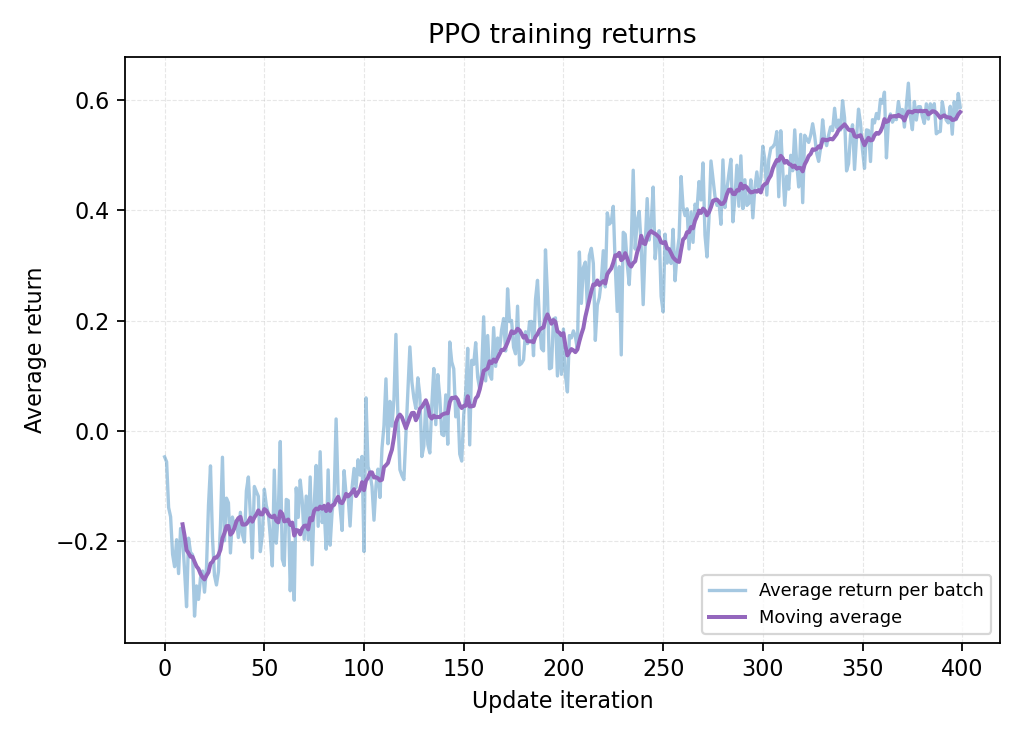
\includegraphics[width=0.8\linewidth]{ppo_returns.png}
  \caption{PPO 训练回报及滑动平均}
  \label{fig:ppo_returns_cn}
\end{figure}

\begin{figure}[H]
  \centering
  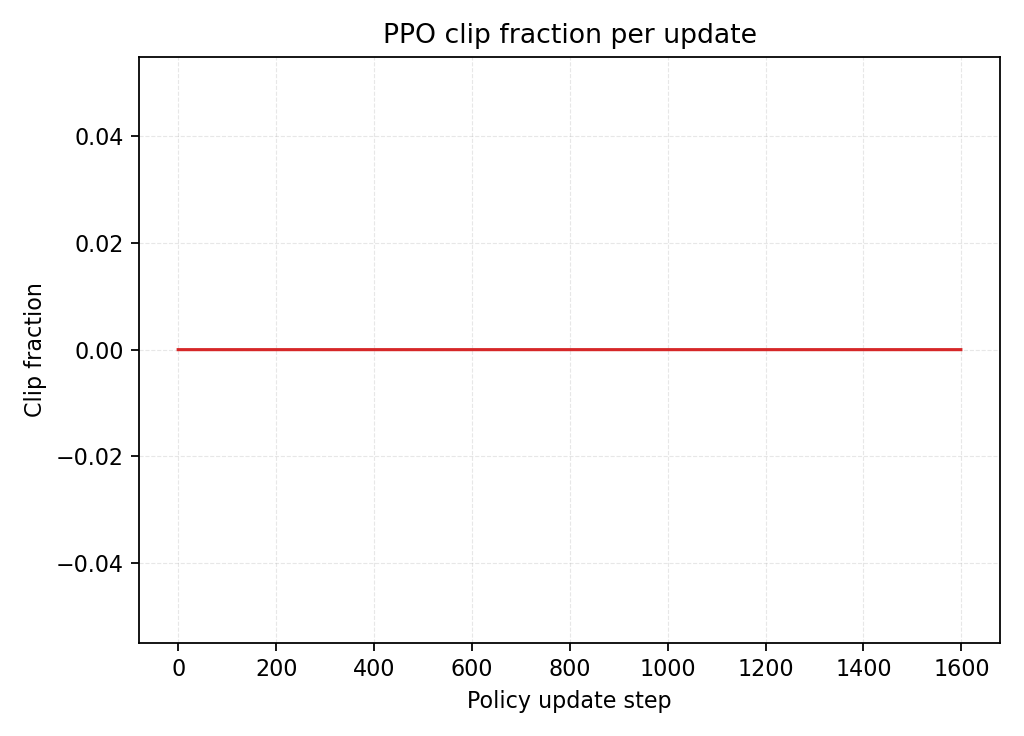
\includegraphics[width=0.82\linewidth]{ppo_clip_stats.png}
  \caption{每次更新的 clip fraction,反映被裁剪比例}
  \label{fig:ppo_clip_stats_cn}
\end{figure}

\FloatBarrier
\section{总结}
PPO 通过裁剪概率比率实现简洁而稳定的策略优化。优势归一化、熵正则和对 clip/KL 统计的监控有助于保持收敛稳定性。示例说明了回报稳步提升且裁剪比例保持在合理范围。

\end{document}